\documentclass[../main.tex]{subfiles}

\begin{document}

    Zarządzanie testowaniem.
    \begin{itemize}
        \item Zarządzanie strategicznie,
        \item Zarządzanie operacyjne,
        \item Zarządzanie zespołem testowym.
    \end{itemize}

    \subsection{Testowanie oparte na ryzyku.}

    \textbf{Ryzyko} – możliwość (prawdopodobieństwo) wystąpienia negatywnego lub niepożądanego zdarzenia.

    \textbf{Poziom ryzyka} – ważność ryzyka określona przez prawdopodobieństwo i wpływ; może być ilościowy lub
    jakościowy.

    \textbf{Zarządzanie ryzykiem} - w podejściu opartym na ryzyku ryzyko jest podstawową bazą testów.

    \begin{figure}[H]
        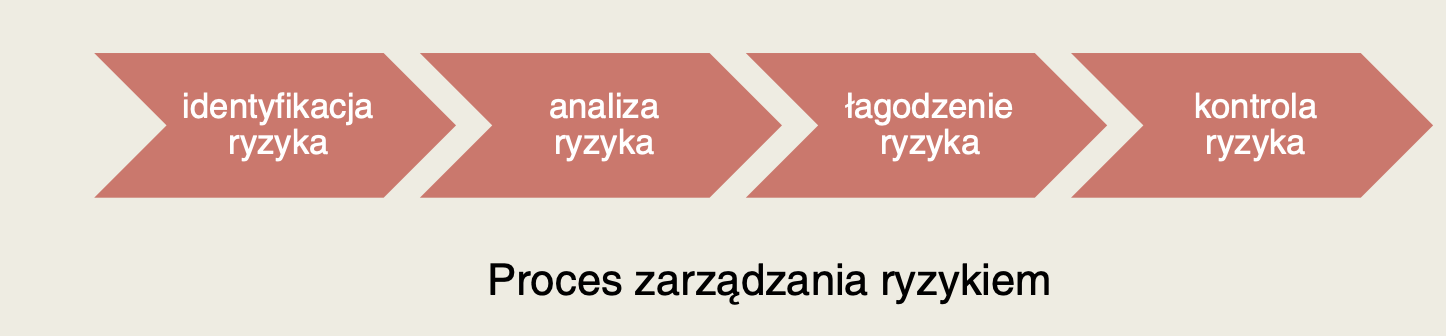
\includegraphics[width=\linewidth]{ryzyko.png}
    \end{figure}

    \textbf{Identyfikacja ryzyka} - proces identyfikacji możliwych do wystąpienia ryzyk. Techniki identyfikacji
    ryzyka:
    \begin{itemize}
        \item burza mózgów
        \item listy kontrolne
        \item historia awarii
        \item wywiady eksperckie
        \item szablony ryzyk
        \item niezależna ocena
        \item doświadczenie z poprzednich projektów
    \end{itemize}


    \textbf{Łagodzenie ryzyka} - proces implementacji planów mających zapobiegać ryzyku. Metody łagodzenia ryzyka:
    \begin{itemize}
        \item łagodzenie ryzyka (risk mitigation) przez podjęcie czynności prewencyjnych, zapobiegających pojawieniu się ryzyka lub zmiejszających ich ewentualną dotkliwość
        \item plany awaryjne (contingency plans) mające na celu redukcję siły oddziaływania ryzyka, które wystąpi
        \item transfer ryzyka (risk transfer), czyli przeniesienie ryzyka na stronę trzecią (np. ubezpieczyciela), który ponosi skutki wystąpienia ryzyka
        \item zignorowanie i zaakceptowanie ryzyka, czyli niepodejmowanie żadnych akcji do mommentu wystąpienia ryzyka
    \end{itemize}
    Podczas fazy łagodzenia ryzyka następuje priorytetyzacja testów wg poziomu ryzyka. Poziom ryzyka wpływa na zakres testowania.

    \textbf{Kontrola (monitorowanie) ryzyka} - ciągła obserwacja aktualnego stanu systemu Przykładowe metryki zbierane w ramach procesu:
    \begin{itemize}
        \item \% pokrytych wymagań
        \item \% pokrytych funkcjonalności
        \item \% testów zdanych/nie zdanych
        \item poziom zminimalizowanego i rezydualnego ryzyka
        \item ryzyka w podziale na:
        \begin{itemize}
            \item zminimalizowane (odpowiadające testy przeszły)
            \item "w trakcie" (wykryto problemy)
            \item niepokryte (nie uruchomiono jeszcze odpowiadających testów)
        \end{itemize}
    \end{itemize}


    \subsubsection{Analiza ryzyka}
    Proces oceny zidentyfikowanych ryzyk w celu oszacowania ich wpływu
    oraz prawdopodobieństwa wystąpienia. Wyjście: lista ryzyk z przypisanymi poziomami/priorytetami ryzyk, określeniem zakresu testowania, metod zapobiegania ryzykom na podstawie oceny czynników technicznych i biznesowych poziomu ryzyka
    Metody analizy ryzyka:
    \begin{itemize}
        \item \textbf{FMEA (Failure Mode and Effect Analysis)} - podejście do systematycznej identyfikacji możliwych awarii systemu\\
        Awarie są priorytetyzowane wg:
        \begin{itemize}
            \item konsekwencji ich wystąpień
            \item prawdopodobieństwa(częstości)wystąpień – łatwości ich wykrycia
        \end{itemize}
        Cel FMEA: podjęcie akcji w celu eliminacji lub redukcji awarii, poczynając od najpoważniejszych
        \item \textbf{FTA} (Fault Tree Analysis) (analiza drzewa usterek) - Metoda analizy niezawodności, bezpieczeństwa i utrzymywalności
        Dedukcyjna procedura używana w celu określenia różnych kombinacji awarii software’u, hardware’u i błędów ludzkich, które mogą wywołać niepożądane efekty na poziomie systemowym
        Podejście top-down (od ogółu – awarii systemowej, do szczegółu – pojedynczych błędów na niskich poziomach). Podstawowe elementy to bramki logiczne.
        \item \textbf{QFD} (Quality Function Deployment)
        \item \textbf{PRisMa} (Product Risk Management) - prawdopodobieństwo i wpływ traktowane osobno, nie łącznie
    \end{itemize}

    \begin{figure}[H]
        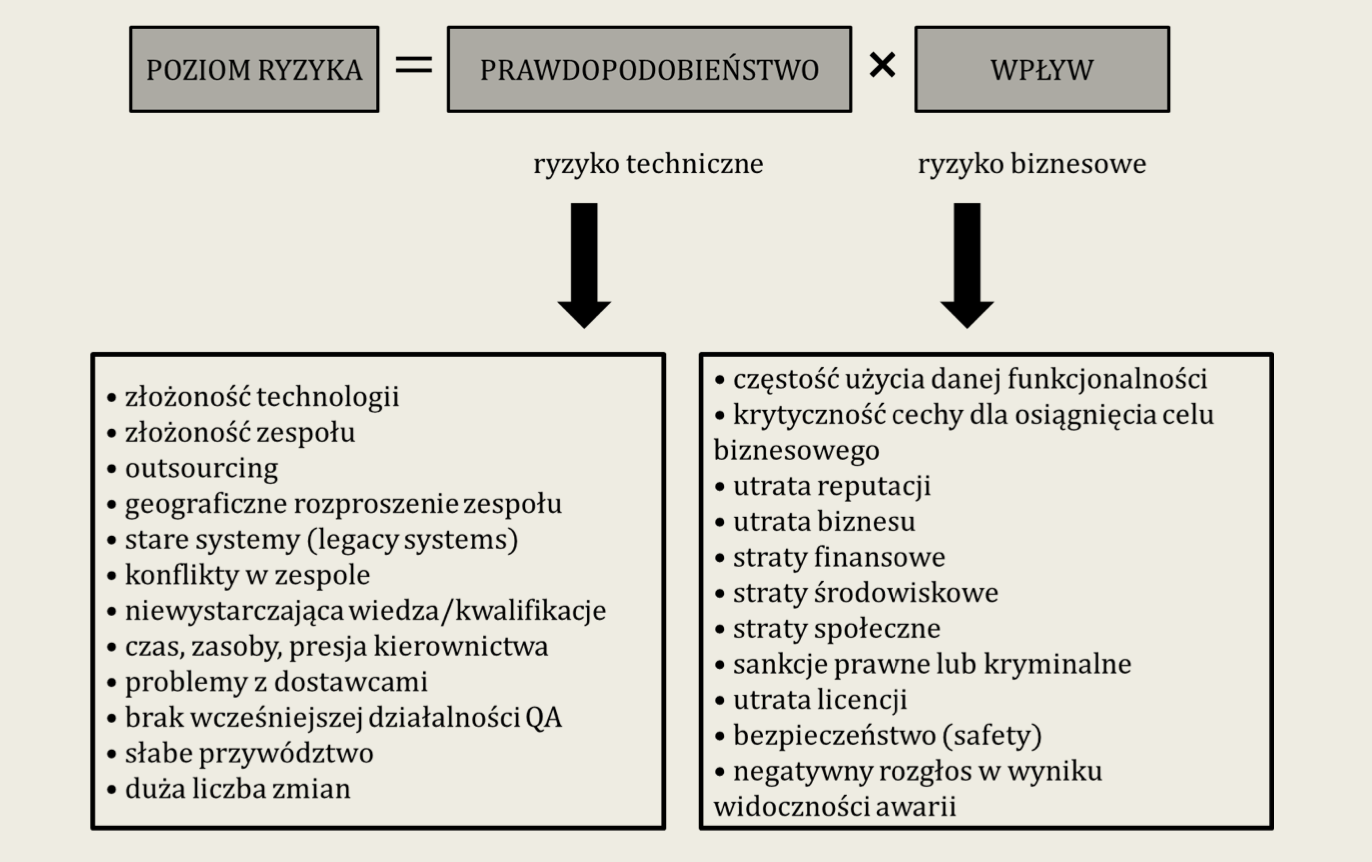
\includegraphics[width=\linewidth]{analiza_ryzyka.png}
    \end{figure}

    \textbf{Ilościowa i jakościowa analiza ryzyka}.

    Szacowanie ilościowe - określenie kosztu materializacji ryzyka. Często trudne lub niemożliwe – wtedy stosuje się podejście jakościowe.


    \subsubsection{Biznesowa wartość testowania.}

    \textbf{Model CoQ} (Cost of (Poor) Quality) - model opisujący koszty związane z dostarczeniem
    produktu lub usługi o niskiej jakości.
    Rodzaje kosztów

    \begin{table}[h]
\begin{center}
    \begin{tabular}{| p{5cm} | p{10cm} |}
        \hline
        \textbf{Rodzaj kosztów} & \textbf{Powód ich ponoszenia}\\
        \hline
        \hline
        koszty \textbf{zapobiegania} & aby unikać defektów; dot. wymagań, planowania i zapewniania jakości, szkoleń (np. szkolenie deweloperów, aby pisany kod był lepszej jakości)\\
        \hline
        koszty \textbf{wykrywania} & aby wykrywać defekty; ponoszone nawet, gdy nie wykryjemy żadnych defektów (np. wydatki na analizę, projektowanie, implementację, niektóre koszty wykonania testów)\\
        \hline
        koszty \textbf{wewnętrznego błędu} & z powodu wykrycia awarii (np. pozostałe koszty wykonania testów, koszty re-testów, koszt naprawy defektu przez programistę)\\
        \hline
        koszty \textbf{zewnętrznego błędu} & z powodu niewykrycia awarii (np. koszty wsparcia technicznego, helpdesku, naprawy defektów polowych, kary umowne)\\
        \hline
    \end{tabular}
\end{center}
\end{table}

\end{document}